\documentclass[12pt]{article}
\usepackage[utf8]{inputenc}
\usepackage[brazil]{babel}
\usepackage{natbib}  % Asegúrate de que esté esta línea
\bibliographystyle{apalike}  % Añade esto en el preámbulo
\usepackage{amsmath}
\usepackage{graphicx}
\usepackage{natbib}
\usepackage{geometry}
\usepackage{booktabs}
\usepackage{hyperref}
\usepackage{caption}  % Añadir al preámbulo
\geometry{margin=2.5cm}
\setlength{\parindent}{0pt}

\title{Cálculo de $L_{inv}$ e Classificação da Estabilidade Atmosférica}
\author{}
\date{}

\begin{document}

\maketitle

% ------------------------- INTRODUÇÃO -------------------------
\section{Introdução}
A estabilidade atmosférica na camada limite superficial é um fator essencial para otimizar operações relacionadas à energia eólica sobre o oceano. Este relatório apresenta uma metodologia para estimar a frequência climatológica de condições \textbf{estáveis, instáveis e neutras} por meio do cálculo da longitude inversa de Obukhov (\(L_{inv}\)). Os resultados permitem identificar padrões horários e mensais na região costeira do Brasil (-21.6389°, -40.8693°) de interesse. Os cálculos e a lógica da estimativa estão detalhados no repositório GitHub: \url{https://github.com/Japq91/Obukhov/}
% ------------------------- FUNDAMENTOS TEÓRICOS -------------------------
\section{Fundamentos Teóricos}

\subsection{Comprimento de Obukhov na Camada Limite}
De acordo com \citep{ecmwf_ifs_cy49r1_physics}, o comprimento de Obukhov ($L$) é um parâmetro que caracteriza os efeitos da flutuabilidade na turbulência atmosférica próxima à superfície. Ele é definido como:
\begin{equation}
L = -\frac{u_*^3 \theta_v}{k g \overline{w'\theta_v'}}
\end{equation}

Onde:
\begin{itemize}
    \item $u_*$: Velocidade de fricção (calculada no script \texttt{obukhov\_calculate.py})
    \item $\theta_v$: Temperatura potencial virtual (derivada de \texttt{t2m} e \texttt{d2m} do ERA5)
    \item $\overline{w'\theta_v'}$: Fluxo de calor sensível (variável \texttt{ishf} do ERA5)
    \item $k = 0.4$: Constante de von Kármán
\end{itemize}

\subsection{Interpretação Física}
Segundo \citep{ecmwf_obukhov_era5_guide}, os valores de $L$ definem três regimes:
\begin{itemize}
    \item \textbf{Instável} ($L < 0$): condições convectivas com fluxo ascendente de calor da superfície. Favorece a turbulência por flutuabilidade. Dominado por convecção (associado a dias ensolarados).
    \item \textbf{Estável} ($L > 0$): estratificação térmica estável com fluxo descendente de calor. Inibe a mistura vertical (associado a noites claras).
    \item \textbf{Neutro} ($|L| \to \infty$): ausência de troca de calor sensível ($\overline{w'\theta'} \approx 0$), a turbulência é gerada apenas por cisalhamento.
\end{itemize}

\subsection{Implementação Numérica}
No código, calcula-se o comprimento de Obukhov na forma inversa ($L_{inv} = 1/L$) para evitar problemas numéricos com valores extremos ($L \to \infty$), normalizando esses casos para zero:
\begin{equation}
L_{inv} = \frac{vk \cdot g \cdot tv_{*}}{tv_2 \cdot u_*^2}
\end{equation}

Essa equação corresponde à linha 78 do script \texttt{obukhov\_calculate.py}, e utiliza as seguintes variáveis:
\begin{itemize}
    \item $vk$: Constante de von Kármán (0.4)
    \item $g$: Aceleração da gravidade (9.81 m/s²)
    \item $tv_{*} = -wtv / u_*$: Escala de temperatura virtual turbulenta
    \item $tv_2 = T_{2m}(1 + 0.6078 \cdot q_2)$: Temperatura virtual a 2 metros
    \item $u_*$: Velocidade de fricção, calculada como:
    \[
    u_* = \sqrt{\frac{\tau}{\rho}}, \quad \tau = \sqrt{u_{\tau,x}^2 + u_{\tau,y}^2}
    \]
    com \texttt{iews} e \texttt{inss} como componentes do estresse superficial, e $\rho = \frac{p}{R_d \cdot tv_2}$ como densidade do ar
    \item $wtv = w_t + \text{retv} \cdot T_{2m} \cdot w_q$: Fluxo turbulento de temperatura virtual
\end{itemize}

As variáveis de entrada são provenientes do ERA5: temperatura (\texttt{t2m}), temperatura de orvalho (\texttt{d2m}), pressão de superfície (\texttt{sp}), fluxos de calor sensível (\texttt{ishf}) e latente (\texttt{ie}), e componentes do estresse superficial (\texttt{iews}, \texttt{inss}).

\subsection{Limitações do Cálculo}
\label{subsec:limitacoes}

Em áreas com orografia significativa, o valor de $L_{inv}$ pode ser menos confiável devido a:
\begin{itemize}
    \item A teoria da similaridade de Monin-Obukhov perde validade em terrenos complexos, conforme discutido por \citep{stull1988}.
    \item Os fluxos de momento no ERA5 incluem contribuições parametrizadas da orografia sub-resolvida (esquema TOFD*) \citep{beljaars2004}.
\end{itemize}

O ECMWF recomenda restringir o uso de $L_{inv}$ a áreas onde o parâmetro \texttt{sdfor} (desvio padrão da orografia subgrid) seja inferior a 50 m, pois nestas regiões a contribuição do TOFD* para o estresse turbulento é mínima.

\textit{*TOFD: Turbulent Orographic Form Drag scheme}
% ------------------------- METODOLOGIA -------------------------
\section{Metodologia}
\subsection{Navegação no Repositório GitHub}

O repositório está estruturado para facilitar o cálculo do comprimento de Obukhov e a classificação da estabilidade atmosférica. As seções mais relevantes são resumidas a seguir:

\begin{itemize}
    \item \textbf{Scripts principais} (\texttt{cods/}):
    \begin{itemize}
        \item \texttt{obukhov\_calculate.py}: Calcula $L_{inv}$ e $u_*$ a partir de arquivos NetCDF do ERA5.
        \item \texttt{save\_events.py}: Classifica condições de estabilidade (estável, instável, neutra) e exporta os resultados em formato CSV.
        \item \texttt{plot\_point.py}: Visualiza climatologias horárias e mensais (Figuras 1a, 1b, 1c).
    \end{itemize}

    \item \textbf{Diretórios de entrada/saída}:
    \begin{itemize}
        \item \texttt{dados/}: contém os arquivos NetCDF de entrada com variáveis meteorológicas do ERA5.
        \item \texttt{out\_nc/}: armazena arquivos NetCDF com $L_{inv}$ e $u_*$.
        \item \texttt{out\_csv/}: contém resultados classificados por condição de estabilidade (estável/instável/neutra).
    \end{itemize}

    \item \textbf{Classificação da estabilidade atmosférica}:
    \begin{itemize}
        \item \texttt{Linv < -0.01} $\Rightarrow$ Instável
        \item \texttt{Linv > 0.01} $\Rightarrow$ Estável
        \item \texttt{-0.01 $\leq$ Linv $\leq$ 0.01} $\Rightarrow$ Neutra
    \end{itemize}
\end{itemize}

% ------------------------- RESULTADOS -------------------------
\section{Resultados Climatológicos}
\subsection{Distribuição Horária e Mensal}
%%%
\begin{center}
    \begin{minipage}{0.49\textwidth}
        \centering
        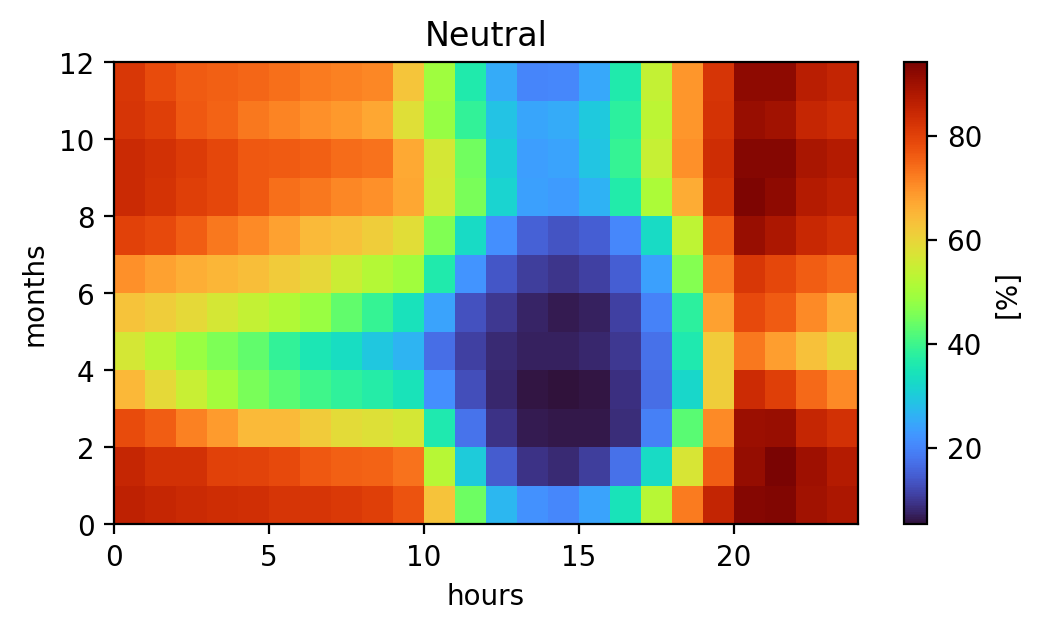
\includegraphics[width=\linewidth]{neutral_35years.png}
    \end{minipage}
    \hfill
    \begin{minipage}{0.49\textwidth}
        \centering
        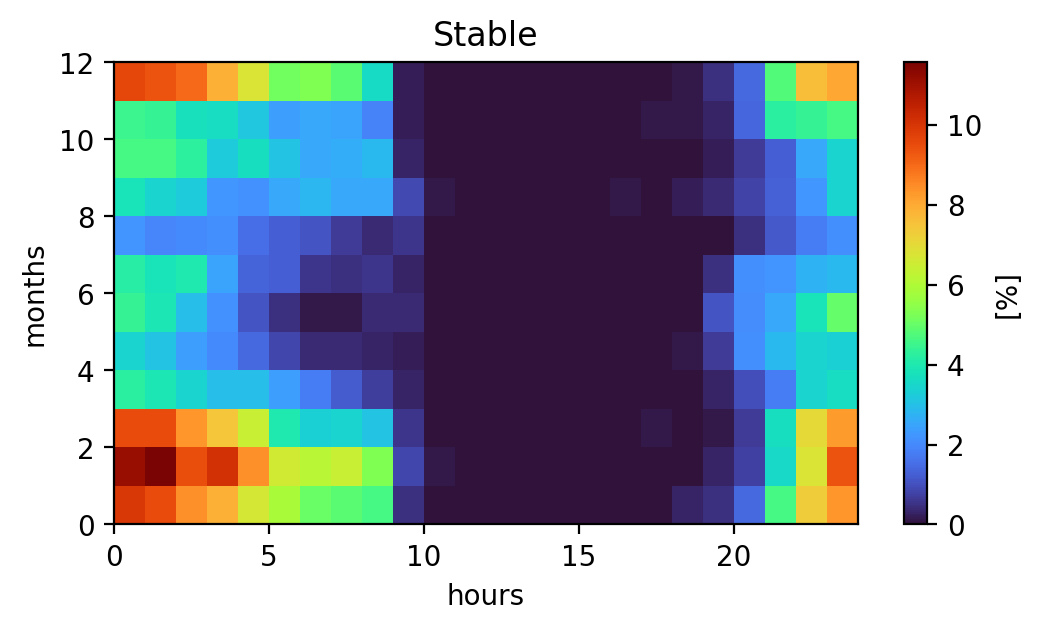
\includegraphics[width=\linewidth]{stable_35years.png}
    \end{minipage}

    \vspace{0.5cm}
    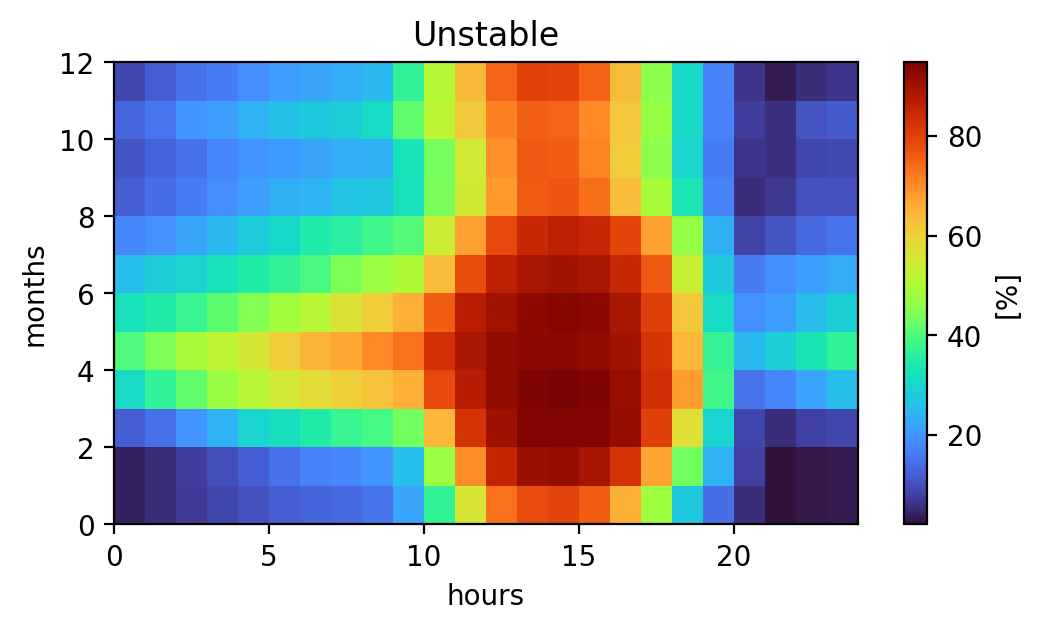
\includegraphics[width=0.49\textwidth]{unstable_35years.png}
    
    \captionof{figure}{Distribuição mensal/horária das condições de estabilidade atmosférica (1990–2024). Eixo X: Hora do dia (UTC), Eixo Y: Mês.}
    \label{fig:clima}
\end{center}
%%%%
\begin{itemize}
    \item \textbf{Condições Instáveis}: Máximos entre 10:00–18:00 UTC (Figura 1c), associados ao aquecimento solar. Estacionalmente, maior ocorrência entre janeiro e agosto.
    \item \textbf{Condições Estáveis}: Maior frequência entre 23:00 e 04:00 UTC. Predomina a baixa frequência dessas condições principalmente entre 09:00 e 20:00 durante todo o ano (Figura 1b).
    \item \textbf{Condições Neutras}: Picos após as 19:00 UTC (Figura 1a), favorecidos pelo resfriamento radiativo. Frequência mais alta de agosto até fevereiro.
\end{itemize}


%% ------------------------- RELEVANCIA PARA PETROBRAS -------------------------
% Estos patrones permiten:
% \begin{itemize}
%     \item Programar mantenimiento en períodos estables/nocturnos.
%     \item Maximizar generación en horas neutras/inestables.
%     \item Evitar daños por turbulencia extrema.
% \end{itemize}

% ------------------------- REFERENCIAS -------------------------

\bibliographystyle{apalike}  % Solo aquí, sin duplicados
\bibliography{latex22}         % Nombre de tu archivo .bib
\end{document}